%\documentclass{article}
\documentclass[twocolumn]{article}

\title{Two Approaches to the String Wrapping Problem}
\author{Will Bolton}
\date{\today}
%\usepackage[hmargin=2.5cm,vmargin=2.5cm]{geometry} %Favourite. From 390 year 2
\usepackage[textwidth=16cm,textheight=23cm]{geometry} %Nadia's
\usepackage{graphicx}
\usepackage{natbib}
\usepackage{amsmath}
\usepackage{amssymb}
\usepackage{amsfonts}
\usepackage{tikz}
\usepackage{booktabs}
\usepackage{color}
%\usepackage[lofdepth,lotdepth]{subfig} %difference between this and caption/subcaption??
\usepackage{tikz}
\usepackage{cleveref}
\usepackage{lipsum}
\usepackage{todonotes}
\usepackage{microtype}
\usepackage{enumerate}
\usepackage{listings}
\usepackage{caption}
\usepackage{subcaption}

% format for defining new environments:
% \newenvironment{ <<name>> }{ <<starting text/formatting rules>> }{ <<finishing text/formatting rules>> }

%Proof environment
\newenvironment{proof}
 {
   \begin{trivlist} %This new environment uses a list environment to handle spacing etc.
     \item[] {\bf Proof.} %This starts a new list item and inserts the title ``Proof.'' in bold
 }
 {
    \nolinebreak    %this stops a new line being inserted after proof before qed mark
    \hfill          %this expands to the end of the line, pushing the QED mark to the right margin
    \rule{2mm}{2mm} %this is the QED mark (small black square)
   \end{trivlist}
 }
 
 %sketch of proof environment
 \newenvironment{sproof}
 {
   \begin{trivlist}
     \item[] {\bf Sketch of proof.}
 }
 {
    \nolinebreak
    \hfill
    \rule{2mm}{2mm}
   \end{trivlist}
 }
 
 %Definition environment
\newenvironment{definition}
 {
   \begin{trivlist}
     \item[] {\bf Definition.}
 }
 {
   \end{trivlist}
 }
 
 
%Theorem environment (this is a bit different because there is a \newtheorem command)
%Syntax \newtheorem{ <<name>> }{ <<Displayed Title>> }[ <<Where to take numbering from>> ]
\newtheorem{theorem}{Theorem}[subsection] %this defines a new theorem environment ``theorem'' and numbers it within subsections
\newtheorem{lemma}{Lemma}[subsection]     %Lemma environment
\newtheorem{proposition}{Proposition}[subsection]
\newtheorem{corollary}{Corollary}[subsection]

%Two very useful commands
%Command syntax \newcommand{ <<name>> }[ <<number of arguments>> ]{ <<command content>> } #1, #2 etc mark where arguments are inserted

%Differential - This is upright d (\rm means ``roman'' i.e. upright font). The rest of the command handles spacing.
\newcommand{\ud}{\, {\rm d} \kern-.015em }

%This is bold in math mode, and works for letters, numbers and greek (\mathbf doesn't work for greek).
\newcommand{\bm}[1]{\mbox{\protect\boldmath $ #1 $}}




%\usepackage{kpfonts}

\begin{document}
\maketitle

\section{Problem}
A cylinder of length 12 units and circumference 4 units has a piece of string wrapped perfectly around it, such that it completes exactly 4 revolutions of the body. The task is to find the length of the string. This is visualised in \cref{initial}.

\begin{figure}[htpb] %3D is impossible with my current TikZ abilities, so I've gone for 2D. Asymptote might work for a better figure
\centering
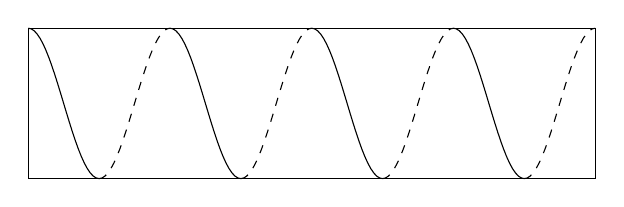
\begin{tikzpicture}[xscale=0.6,yscale=1.5] % scale for twocolumn
%cylinder side on
\draw (0,2/pi) -- (12,2/pi) -- (12,-2/pi) -- (0,-2/pi) -- (0,2/pi);
%string
%first section
\draw[domain=0:1.5] plot (\x, {2/pi*cos(2*pi*\x/3 r)});
%second section
\draw[dashed, domain=1.5:3] plot (\x, {2/pi*cos(2*pi*\x/3 r)});
%third section
\draw[domain=3:4.5] plot (\x, {2/pi*cos(2*pi*\x/3 r)});
%fourth section
\draw[dashed, domain=4.5:6] plot (\x, {2/pi*cos(2*pi*\x/3 r)});
%fifth section
\draw[domain=6:7.5] plot (\x, {2/pi*cos(2*pi*\x/3 r)});
%sixth section
\draw[dashed, domain=7.5:9] plot (\x, {2/pi*cos(2*pi*\x/3 r)});
%seventh section
\draw[domain=9:10.5] plot (\x, {2/pi*cos(2*pi*\x/3 r)});
%eigth section
\draw[dashed, domain=10.5:12] plot (\x, {2/pi*cos(2*pi*\x/3 r)});
\end{tikzpicture}
\caption{Side on view of the problem}
\label{initial}
\end{figure}

\section{Sensible approach}
The sensible approach is to realise that unrolling the cylinder simplifies the computation greatly; once this is done, a simple application of Pythagoras' theorem gives the length of the string as $4\times \sqrt{3^2+4^2}=4\times 5=20$. This is because each revolution corresponds to the hypotenuse of a right-angled triangle with sides of length 4 (from the circumference) and 3 (horizontal distance along cylinder; 4 revolutions with 12 units travelled $\Rightarrow 12/4=3$ units per revolution). \Cref{sensible} depicts the situation.
\begin{figure}[htpb]
\centering
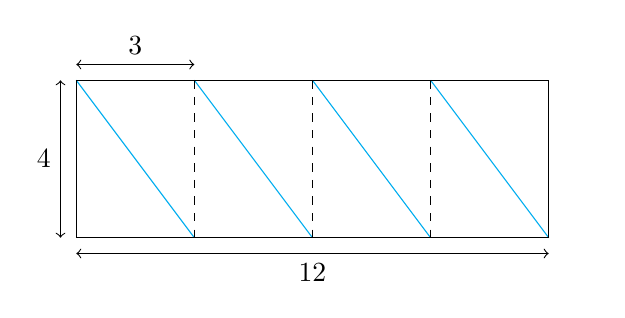
\begin{tikzpicture}[scale=0.5] % scale for twocolumn
%lines
\draw [cyan] (0,0) -- (3,-4);
\draw [cyan] (3,0) -- (6,-4);
\draw [cyan] (6,0) -- (9,-4);
\draw [cyan] (9,0) -- (12,-4);
%rectangle
\draw (0,0) -- (12,0) -- (12,-4) -- (0,-4) -- (0,0);
%guidelines
\draw [dashed] (3,0) -- (3,-4);
\draw [dashed] (6,0) -- (6,-4);
\draw [dashed] (9,0) -- (9,-4);
%labels
\draw [<->] (0,-4.4) -- (12,-4.4);
\node [below] at (6,-4.4) {12};
\draw [<->] (0,0.4) -- (3,0.4);
\node [above] at (1.5,0.4) {3};
\draw [<->] (-0.4,0) -- (-0.4,-4);
\node [left] at (-0.4,-2) {4};
%for balanced centering
\draw [white, <->] (12.4,0) -- (12.4,-4);
\node [white, right] at (12.4,-2) {4};
\end{tikzpicture}
\caption{The easy way to solve the string wrapping problem on the unrolled cylinder}
\label{sensible}
\end{figure}

\section{More fun approach}
Alternatively, we can use the techniques developed in \texttt{MATH329} to solve the problem more directly; that is, without unrolling the cylinder. Ensuring that the centre of the cylinder lies along the z~axis, we let the string be represented by a curve in $\mathbb{R}^3$ that will take the form
$$\bm{\gamma}(t): (0,12) \rightarrow \mathbb{R}^3;\ t \mapsto (r\sin{at}, r\cos{at}, t),$$
where $r$ is the radius of the cylinder and $a$ is a constant to be determined.

Since the circumference of the cylinder is known to be 4, it follows that $r=4/2\pi=2/\pi$. Considering $a$, we know that multiplication by $a$ in the trigonometric functions divides the period by $a$. Since we need the period to equal 3,
\begin{align*}
3&=2\pi/a\\
\Rightarrow a&=2\pi/3
\end{align*}
Thus
$$\bm{\gamma}(t): (0,12) \rightarrow \mathbb{R}^3;\ t \mapsto (\frac{2}{\pi}\sin{\frac{2\pi}{3}t}, \frac{2}{\pi}\cos{\frac{2\pi}{3}t}, t)$$
The difficult work is done. Now all that's left is to apply the arc-length formula:
\begin{equation}
\ell(\vec{ab})=\int_a^b |\bm{\gamma}'|\ud t
\label{arclength}
\end{equation}
First, we differentiate $\bm{\gamma}$:
$$\bm{\gamma}'(t): (0,12) \rightarrow \mathbb{R}^3;\ t \mapsto (\frac{4}{3}\cos{\frac{2\pi}{3}t}, -\frac{4}{3}\sin{\frac{2\pi}{3}t}, 1)$$
Now apply \cref{arclength}:
\begin{align*}
\ell&=\int_0^{12} \sqrt{\frac{4^2}{3^2} \left(\cos^2{\frac{2\pi}{3}t}+\sin^2{\frac{2\pi}{3}t} \right)+1^2} \ud t \\
&=\int_0^{12} \sqrt{\frac{4^2}{3^2}+\frac{3^2}{3^2}} \ud t \\
&=12\times \frac{5}{3} = 20
\end{align*}
So we arrive at the same answer as before, namely that the string is 20 units long.
\end{document}